\chapter{User research, elicitación y análisis preliminar de requerimientos}

\section{Propósito del capítulo}

Este capítulo interpreta el relevamiento realizado con profesionales de diagnóstico por imágenes y lo transforma en insumo de producto, siguiendo la cadena entrevistas, hallazgos, necesidades, requerimientos y épicas. El registro textual de las entrevistas se conserva en el Anexo D. No constituye una validación clínica: documenta una etapa exploratoria y justifica decisiones de alcance que el Capítulo 9 formaliza.
% CROSS_REFERENCE_MAPPING_REQUIRED
% CROSS_REFERENCE_MAPPING_REQUIRED

\section{Diseño del relevamiento}

El relevamiento se organizó mediante entrevistas semiestructuradas, técnica recomendada en las etapas exploratorias del diseño centrado en el usuario porque combina la comparabilidad de una guía común con la posibilidad de profundizar en aspectos no previstos \parencite{goodman_observing_user_experience_2012}. Se utilizó una guía común de preguntas, pero se permitió repreguntar y profundizar según la experiencia de cada profesional. El objetivo no fue validar clínicamente un sistema terminado, sino identificar criterios tempranos de utilidad, confianza, alcance y riesgo para orientar el diseño del MVP.

Ejes de entrevista y objetivos:

\begin{itemize}
  \item Flujo actual de trabajo. Comprender cómo se revisa una RM lumbar y cómo se llega al informe.
  \item Planos y secuencias. Identificar el rol del plano sagital, axial, coronal y de secuencias como T1, T2 o STIR.
  \item Hallazgos relevantes. Detectar estructuras, signos y mediciones consideradas útiles.
  \item Errores críticos. Comprender fallas clínicamente graves o inaceptables.
  \item Interfaz y confianza. Explorar qué debe mostrar el sistema para ser usable y confiable.
  \item Validación. Indagar contra qué debería validarse: expertos, segmentaciones manuales, métricas o uso profesional.
  \item Alcance defendible. Identificar qué incluir, excluir o diferir para evitar sobreprometer capacidades.
  \item Comparación temporal. Explorar el valor de relacionar estudios actuales y previos del mismo sujeto.
\end{itemize}

La muestra es intencional y exploratoria. No busca representatividad estadística de toda la comunidad radiológica. Su valor reside en contrastar perfiles con experiencia directa en RM, informe, segmentación, control de calidad y patología de columna.

\section{Perfil de profesionales entrevistados}

EN-01 — Dra. Susana Torres (Matrícula Nacional 179537). Médica radióloga con experiencia en resonancia magnética, segmentación y control de calidad. Referencias mencionadas: Sociedad Argentina de Radiología, FLENI y Prenuvo. Duración aproximada: 22 minutos.

EN-02 — Dr. Gonzalo Brito (Matrícula Provincial 96798). Médico radiólogo que informa resonancia magnética, tomografía y ecografía. Institución o referencia informada: Imágenes MDQ. Duración aproximada: 29 minutos.

EN-03 — Dra. Claudia Cejas. Médica radióloga, especialista en patología neuromuscular y de columna. Referencias mencionadas: FLENI y Sociedad Argentina de Radiología. Duración aproximada: 33 minutos.

EN-04 — Dr. Bruno Bregonzi. Profesional que informa un volumen elevado de resonancias, con práctica frecuente en columna lumbar y población deportiva. La institución y la duración no fueron especificadas en la transcripción provista. La entrevista fue realizada por Enzo Asplanatti y reconstruida a partir de una transcripción automática sin separación de hablantes.

EN-05 — Dr. Eduardo Luis Castiglione. Médico neurorradiólogo con un alto volumen de estudios de columna lumbar, mayoritariamente de patología degenerativa. Aporta una mirada centrada en el contexto clínico de cada hallazgo, en la exactitud del nivel anatómico como base del análisis y en el interés por una interpretación asistida por nivel.

La selección de perfiles permitió contrastar miradas vinculadas con informe de RM, práctica cotidiana en diagnóstico por imágenes, segmentación, control de calidad, patología de columna y adopción de herramientas asistidas por inteligencia artificial. EN-04 agrega una perspectiva de alto volumen de lectura cotidiana y refuerza el valor de una interfaz que funcione como alivio operativo; EN-05, con perfil de neurorradiólogo, aporta el foco en la exactitud del nivel anatómico y en el contexto clínico del hallazgo.

\section{Criterio de tratamiento de las transcripciones}

Las transcripciones completas se incorporan en un anexo independiente en formato de diálogo directo. Para el análisis de este capítulo se utilizan como fuentes primarias, codificadas como EN-01 a EN-05. El capítulo no reproduce las entrevistas completas ni reemplaza el anexo, sino que sintetiza patrones, divergencias y decisiones de producto derivadas del relevamiento.

La cuarta entrevista requiere una salvedad metodológica específica: el archivo de origen no incluía separación de hablantes. Su versión depurada fue reconstruida por contexto conversacional, normalizando términos técnicos evidentes y evitando agregar contenido no presente en la fuente. Por ello, se utiliza como evidencia cualitativa exploratoria y no como transcripción literal palabra por palabra.

\section{Matriz de hallazgos}

{\small
\setlength{\LTleft}{0pt}
\setlength{\LTright}{0pt}
\renewcommand{\arraystretch}{1.18}
\setlength{\tabcolsep}{3pt}
\begin{longtable}{>{\raggedright\arraybackslash}p{0.24\textwidth} >{\raggedright\arraybackslash}p{0.38\textwidth} >{\raggedright\arraybackslash}p{0.30\textwidth}}
\caption{Matriz de hallazgos}\label{tab:user-research-hallazgos}\\
\hline
\textbf{Hallazgo} & \textbf{Evidencia observada} & \textbf{Impacto en el proyecto} \\
\hline
\endfirsthead
\caption[]{Matriz de hallazgos (continuación)}\\
\hline
\textbf{Hallazgo} & \textbf{Evidencia observada} & \textbf{Impacto en el proyecto} \\
\hline
\endhead
\hline
\endfoot
Hallazgo 1 — La IA debe asistir, no diagnosticar de forma autónoma. & EN-01 a EN-05 aceptan el valor de la IA como apoyo, pero mantienen la interpretación y la decisión final en el profesional. & conservar un enfoque human-in-the-loop, con resultados revisables, editables y explícitamente no diagnósticos. \\
Hallazgo 2 — El plano axial es necesario para una evaluación lumbar más completa. & EN-01 indicó que el sagital aislado deja incompleta la evaluación; EN-02 remarcó la importancia de revisar todos los planos; EN-03 recomendó considerar información axial; EN-04 señaló que el axial resulta especialmente importante para lateralidad y relación con raíces y neuroforámenes. & incorporar el plano axial como módulo complementario sin desplazar el núcleo sagital ni afirmar correspondencia tridimensional entre datasets independientes. \\
Hallazgo 3 — La revisión real se realiza sobre múltiples imágenes, secuencias y planos. & los profesionales describieron recorridos que combinan sagital T1, sagital T2, STIR, axial y, según el caso, coronal u otras secuencias. EN-04 aclaró además que en la práctica puede haber protocolos incompletos por movimiento, claustrofobia o tolerancia del paciente. & evitar reducir conceptualmente el estudio a una única imagen; identificar las secuencias disponibles y comunicar de forma explícita cuando falta un plano o una serie esperada. \\
Hallazgo 4 — La visualización superpuesta aumenta la confianza. & EN-01 pidió poder ver dónde el sistema identifica el hallazgo; EN-03 valoró una salida visual verificable; EN-04 indicó que lo importante es observar la segmentación ya realizada como guía. & priorizar imagen original, máscaras o contornos superpuestos, control de visibilidad y asociación con el resultado correspondiente. \\
Hallazgo 5 — Las mediciones aportan valor cuando son trazables y no sobrecargan la interfaz. & se mencionaron canal, forámenes, discos, área, diámetros, volumen, alineación, ángulos y medidas en distintos ejes. EN-04 destacó las «mediciones puras» y la superposición de imágenes como funciones que podrían liberar trabajo. & asociar cada medición con imagen, estructura, máscara, plano, corte, unidad y estado de revisión, presentándola de manera progresiva y no invasiva. \\
Hallazgo 6 — La corrección o revisión manual es necesaria. & los profesionales plantearon aceptar, corregir, observar o descartar resultados automáticos. EN-04 reforzó que usaría el sistema como referencia inicial y luego revisaría el estudio personalmente. & exigir una acción profesional explícita antes de considerar revisado un resultado. \\
Hallazgo 7 — El falso negativo y la infravaloración son riesgos críticos. & EN-02 y EN-03 destacaron el peligro de omitir lesiones relevantes; EN-01 señaló el riesgo de sobredimensionar o infravalorar hallazgos. EN-04 ubicó la responsabilidad final en el profesional que informa. & combinar métricas técnicas, comunicación de incertidumbre y revisión obligatoria; no presentar el sistema como garantía de ausencia de patología. \\
Hallazgo 8 — El sistema no debe agregar fricción. & EN-02 advirtió sobre herramientas que agregan pasos o tiempo; EN-04 definió la utilidad en términos de un «alivianador» y pidió que no se muestre información de más. & priorizar simplicidad, tiempos razonables, revelado progresivo de información y mínima carga operativa. \\
Hallazgo 9 — El alcance debe acotarse. & EN-01 y EN-03 recomendaron concentrarse en estructuras o problemas prioritarios; EN-04 sugirió orientarse a un área y comenzar la prueba con un centro o grupo reducido. & mantener foco en región lumbar adulta, segmentación, mediciones, visualización y revisión, sin prometer diagnóstico diferencial amplio. \\
Hallazgo 10 — La comparación con estudios previos posee valor potencial alto. & La mayoría de los entrevistados valoró disponer de estudios anteriores. EN-04 la consideró útil especialmente para seguimiento; se mantiene como evolución de producto. & conservar una referencia de sujeto de-identificada y diseñar la evolución longitudinal como comparación descriptiva futura, sin afirmar porcentajes clínicos no validados. \\
Hallazgo 11 — La identificación correcta del nivel anatómico condiciona la utilidad del resultado automático. & Señalado principalmente por EN-05 (neurorradiólogo): la utilidad del resultado depende de ubicar correctamente el nivel, y el contexto clínico condiciona su interpretación. & reforzar la localización por nivel, la trazabilidad del hallazgo hacia su nivel y corte de origen, y la revisión profesional obligatoria de la salida. \\
\hline
\end{longtable}
}

\section{Lectura analítica de los hallazgos}

Los hallazgos de la Tabla~\ref{tab:user-research-hallazgos} admiten una lectura en cinco criterios de diseño, que el resto del documento retoma como decisiones.

Carácter asistivo. El valor esperado no está en reemplazar el criterio médico sino en delimitar, medir y mostrar elementos que luego puedan comprobarse. La revisión profesional no es una precaución agregada al final: forma parte del flujo, y un resultado automático debe conservar su estado, mostrar su origen y admitir una decisión explícita del usuario.

Incorporación del plano axial. El principal ajuste de alcance surge de la necesidad de correlacionar planos. El diseño original centrado en el sagital se mantiene como base por disponibilidad de datos, pero las entrevistas muestran que una evaluación lumbar representativa requiere información axial. El plano axial dejó así de ser una observación del estado del arte para constituir una necesidad funcional detectada en usuarios, y la respuesta técnica fue un módulo axial complementario entrenado y evaluado de forma independiente. Esa implementación no autoriza a interpretar ambos planos como una reconstrucción conjunta.

Trazabilidad verificable. Los profesionales no solicitaron una predicción sino una salida verificable: la confianza aumenta cuando el sistema muestra dónde detectó una estructura, cómo calculó una medición y qué parte puede revisarse. De ese hallazgo, junto con la comprobación de que los volúmenes contienen múltiples cortes, surgió el visor navegable de la serie completa.

Interfaz orientada a aliviar trabajo. EN-04 pide que el sistema funcione como referencia inicial, muestre la segmentación con claridad y evite información innecesaria; EN-02 advierte sobre la fricción operativa. La interfaz aplica revelado progresivo: la imagen y el resultado principal ocupan el centro, y las mediciones, la trazabilidad y los detalles técnicos quedan disponibles sin cubrir la imagen.

Validación en dos planos y contexto clínico. EN-01 destacó la calidad de las anotaciones de referencia y EN-04 señaló que la utilidad práctica debe contrastarse con profesionales que informan estudios, de modo que la validación separa la evaluación del modelo, la del artifact y el runtime, la de integración y la de usabilidad. Las entrevistas muestran además que la imagen no se interpreta de forma aislada: EN-02 describió los estudios previos como fundamentales y EN-04 señaló que la comparación debe considerar si el dolor cambió. El prototipo persiste los estudios con una referencia de sujeto seudonimizada, conforme a la Ley N.º 25.326, para habilitar a futuro esa comparación, sin emitir conclusiones longitudinales automáticas.

\section{Aspectos no consolidados o diferidos}

La siguiente tabla resume los aspectos que, a partir del relevamiento, se decidieron diferir o acotar.

{\small
\setlength{\LTleft}{0pt}
\setlength{\LTright}{0pt}
\renewcommand{\arraystretch}{1.18}
\setlength{\tabcolsep}{3pt}
\begin{longtable}{>{\raggedright\arraybackslash}p{0.25\textwidth} >{\raggedright\arraybackslash}p{0.37\textwidth} >{\raggedright\arraybackslash}p{0.30\textwidth}}
\caption{Aspectos no consolidados o diferidos}\label{tab:user-research-diferidos}\\
\hline
\textbf{Aspecto no consolidado o diferido} & \textbf{Lectura del relevamiento} & \textbf{Decisión} \\
\hline
\endfirsthead
\caption[]{Aspectos no consolidados o diferidos (continuación)}\\
\hline
\textbf{Aspecto no consolidado o diferido} & \textbf{Lectura del relevamiento} & \textbf{Decisión} \\
\hline
\endhead
\hline
\endfoot
Diagnóstico diferencial automático & Aparece como posibilidad de valor, pero depende de clínica, antecedentes y datos no incluidos en el MVP. & Diferir; no forma parte del núcleo del producto. \\
Lesiones medulares, tumorales, infecciosas u oncológicas & Son relevantes y pueden ser críticas, pero requieren datasets, secuencias y validación específicos. & Documentar como riesgo y posible extensión; no prometer detección amplia. \\
Comparación con estudios previos & Fue valorada por varios de los entrevistados (EN-01 a EN-04). & Mantener como épica futura; comenzar por comparación descriptiva de mediciones y advertencias de comparabilidad, no por scoring clínico. \\
Ejecución en nube & Se considera compatible con el flujo y útil para evitar cómputo local pesado. & Evaluarla en arquitectura, privacidad, costos, disponibilidad y seguridad. Google Cloud se documenta como arquitectura objetivo. \\
Protocolos incompletos & EN-04 señaló que no siempre se dispone de todas las secuencias o planos. & Validar inputs, informar faltantes y evitar inventar resultados para datos ausentes. \\
Alcance degenerativo frente a alcance amplio & Se recomienda acotar a región lumbar adulta, patología discal, estructuras y mediciones prioritarias. & Mantener foco lumbar y separar hallazgos estructurales de conclusiones clínicas. \\
Procesamiento de series o modalidades no soportadas & El relevamiento fundamenta la revisión del estudio completo; la compatibilidad de una serie con un modelo depende de su plano y ponderación. & No ejecutar inferencia automática fuera del alcance validado del modelo; mantener esas series disponibles para revisión visual (view-only). La segmentación full-series se aplica a las series y modalidades soportadas. \\
\hline
\end{longtable}
}

\section{User persona preliminar}

{\small
\setlength{\LTleft}{0pt}
\setlength{\LTright}{0pt}
\renewcommand{\arraystretch}{1.18}
\setlength{\tabcolsep}{3pt}
\begin{longtable}{>{\raggedright\arraybackslash}p{0.25\textwidth} >{\raggedright\arraybackslash}p{0.67\textwidth}}
\caption{User persona preliminar}\label{tab:user-persona}\\
\hline
\textbf{Atributo} & \textbf{Detalle} \\
\hline
\endfirsthead
\caption[]{User persona preliminar (continuación)}\\
\hline
\textbf{Atributo} & \textbf{Detalle} \\
\hline
\endhead
\hline
\endfoot
Usuario principal & Médico/a radiólogo/a o profesional de diagnóstico por imágenes con práctica habitual en resonancia magnética lumbar. \\
Contexto de uso & Revisión de estudios de RM lumbar en centros de diagnóstico, instituciones hospitalarias o entornos especializados, con una carga de trabajo que puede incluir numerosos estudios por jornada. \\
Objetivos & Revisar estudios de manera eficiente; identificar estructuras y relaciones anatómicas relevantes; correlacionar planos y secuencias; apoyarse en mediciones trazables; comparar con estudios previos cuando estén disponibles; mantener control profesional sobre la salida. \\
Frustraciones & Alta carga de estudios; riesgo de omitir hallazgos; mediciones manuales repetitivas; protocolos incompletos; herramientas que agregan tiempo; resultados automáticos que no muestran su origen; pantallas sobrecargadas. \\
Necesidades & Visualización clara de la imagen original; navegación entre cortes y planos disponibles; máscaras o contornos superpuestos; corrección y revisión manual; mediciones asociadas a estructuras y cortes; advertencias ante datos faltantes; validación con expertos; salida estructurada editable. \\
Criterio de confianza & El sistema debe mostrar de dónde surge cada resultado, permitir contrastarlo con la imagen y habilitar su aceptación, observación, corrección o descarte. \\
Límite esperado & La herramienta no debe emitir diagnóstico autónomo ni reemplazar el criterio médico. \\
\hline
\end{longtable}
}

\section{Necesidades detectadas}

{\small
\setlength{\LTleft}{0pt}
\setlength{\LTright}{0pt}
\renewcommand{\arraystretch}{1.18}
\setlength{\tabcolsep}{3pt}
\begin{longtable}{>{\raggedright\arraybackslash}p{0.09\textwidth} >{\raggedright\arraybackslash}p{0.57\textwidth} >{\raggedright\arraybackslash}p{0.26\textwidth}}
\caption{Necesidades detectadas}\label{tab:user-research-necesidades}\\
\hline
\textbf{ID} & \textbf{Necesidad detectada} & \textbf{Origen} \\
\hline
\endfirsthead
\caption[]{Necesidades detectadas (continuación)}\\
\hline
\textbf{ID} & \textbf{Necesidad detectada} & \textbf{Origen} \\
\hline
\endhead
\hline
\endfoot
N-01 & Visualizar máscaras o contornos superpuestos sobre la RM original. & EN-01, EN-03, EN-04. \\
N-02 & Permitir aceptar, observar, corregir o descartar resultados automáticos. & EN-01, EN-02, EN-03, EN-04. \\
N-03 & Revisar conjuntamente la información del plano sagital y del axial de manera trazable, utilizando correspondencia geométrica únicamente cuando pueda verificarse. & EN-01, EN-02, EN-03, EN-04. \\
N-04 & Obtener mediciones trazables por estructura, plano, corte y máscara. & EN-01, EN-02, EN-03, EN-04, EN-05. \\
N-05 & Evitar diagnóstico autónomo y mantener revisión profesional. & EN-01, EN-02, EN-03, EN-04, EN-05. \\
N-06 & Validar resultados con especialistas y no solo con métricas técnicas. & EN-01, EN-02, EN-03, EN-04, EN-05. \\
N-07 & Mantener un flujo simple que no agregue tiempo innecesario. & EN-02, EN-04. \\
N-08 & Registrar errores, discrepancias, correcciones u observaciones para mejorar el sistema. & EN-01, EN-02, EN-03. \\
N-09 & Acotar el alcance a región lumbar adulta y hallazgos estructurales prioritarios. & EN-01, EN-03, EN-04. \\
N-10 & Evaluar comparación con estudios previos como extensión futura. & EN-01, EN-02, EN-03, EN-04. \\
N-11 & Informar de manera explícita la ausencia de secuencias, planos o resultados, sin completar artificialmente la información faltante. & EN-04 y criterio de seguridad derivado. \\
N-12 & Navegar el conjunto de imágenes disponible y conservar la relación entre resultado y corte de origen. & síntesis EN-01–EN-05 y hallazgo de navegación. \\
\hline
\end{longtable}
}

\section{Épicas iniciales y criterios de aceptación}

El relevamiento se organizó en diez épicas académicas que estructuran el trabajo desde la perspectiva del producto y de la tesis: user research y evidencia, requerimientos y trazabilidad, gestión de conjuntos de datos, preprocesamiento, segmentación sagital, factibilidad axial, métricas y mediciones, visualización y revisión, salida estructurada editable, y validación y documentación.

Dos de ellas cambiaron de estado durante el desarrollo. La factibilidad axial dejó de ser una evaluación para convertirse en un módulo implementado y evaluado, con las limitaciones que documenta el Capítulo 13. La visualización se amplió con el visor navegable de la serie completa y la asociación de cada resultado con su corte de origen. La numeración de estas épicas es independiente de los bloques del roadmap y de los hitos experimentales del módulo de inteligencia artificial, según se detalla en la sección 12.2.
% CROSS_REFERENCE_MAPPING_REQUIRED
% CROSS_REFERENCE_MAPPING_REQUIRED

Los criterios de aceptación se definen en tres planos: la tesis exige que cada capítulo trace su contenido hasta una fuente; los repositorios exigen que cada incremento cuente con criterio de aceptación y evidencia localizable; y el tablero de trabajo exige que ningún elemento se declare terminado sin ambas condiciones.

\section{Encuesta cuantitativa a profesionales}

Para complementar las entrevistas con evidencia de mayor amplitud, se realizó una encuesta en línea (Google Forms) difundida entre profesionales vinculados al diagnóstico por imágenes y a la patología de columna. Se obtuvieron 167 respuestas.

\subsection{Criterio de inclusión y dimensionamiento de la muestra}

El universo de interés se definió como el conjunto de profesionales que informan o utilizan resonancias magnéticas de columna lumbar en su práctica: médicos radiólogos, neurorradiólogos, especialistas en diagnóstico por imágenes, traumatólogos y neurocirujanos. Se excluyeron las respuestas provenientes de perfiles ajenos a ese grupo, en coherencia con el alcance del proyecto, que se limita al análisis estructural de RM lumbar y no contempla otras regiones anatómicas ni otras modalidades de imagen.

El tamaño muestral se evaluó mediante la expresión habitual para la estimación de una proporción poblacional \parencite{cochran_sampling_techniques_1977}:

\[
n = \frac{z^2 \cdot p \cdot (1 - p)}{e^2}
\tag{10.1}
\]
% CROSS_REFERENCE_NUMBERING_REVIEW_REQUIRED
% EQUATION_NUMBERING_REVIEW_REQUIRED

donde z es el valor crítico de la distribución normal asociado al nivel de confianza, p la proporción esperada y e el margen de error admitido. Se adoptó p = 0,5, valor que maximiza la varianza y produce por lo tanto la estimación más conservadora, y un nivel de confianza del 95 %, al que corresponde z = 1,96.

Bajo el supuesto de población infinita, las 167 respuestas obtenidas corresponden a un margen de error de ±7,6 puntos porcentuales con un nivel de confianza del 95 %. Alcanzar un margen de ±5 puntos porcentuales bajo los mismos supuestos habría requerido 385 respuestas.

Cuando el universo es finito, el margen de error se corrige mediante el factor de población finita:

\[
e = z \cdot \sqrt{\frac{p \cdot (1 - p)}{n}} \cdot \sqrt{\frac{N - n}{N - 1}}
\tag{10.2}
\]
% CROSS_REFERENCE_NUMBERING_REVIEW_REQUIRED
% EQUATION_NUMBERING_REVIEW_REQUIRED

No se identificó una estimación oficial única y suficientemente específica del universo definido (profesionales que informan o utilizan RM lumbar dentro de los perfiles incluidos) que permita establecer un valor N defendible para aplicar la corrección por población finita. Por este motivo se conserva, únicamente como referencia descriptiva, el cálculo bajo supuesto de población grande o infinita. Dado que la muestra es de conveniencia y no probabilística, el margen calculado no debe interpretarse como un intervalo de confianza poblacional estricto, sino como una referencia de precisión teórica bajo muestreo aleatorio simple. Corresponde señalar dos limitaciones metodológicas. La primera es que la muestra es de conveniencia y no probabilística: la encuesta se difundió por canales profesionales y la participación fue voluntaria, de modo que no puede descartarse un sesgo de autoselección hacia profesionales con mayor interés previo en herramientas informáticas de apoyo. La segunda es que el margen de error calculado describe la precisión estadística de las estimaciones bajo un muestreo aleatorio simple, supuesto que esta encuesta no satisface estrictamente. En consecuencia, los resultados se interpretan como una señal cuantitativa complementaria al análisis cualitativo de las entrevistas, con capacidad para confirmar tendencias, y no como una validación estadística poblacional.

\subsection{Resultados}

El perfil de los encuestados se concentra en roles clínicos vinculados a la RM lumbar: residentes o médicos en formación, diagnóstico por imágenes, traumatología de columna y neurocirugía. Casi tres de cada cuatro obtienen las mediciones de forma manual sobre el visor o las estiman visualmente, y solo nueve utilizan un software que ya las calcula. El dato respalda la oportunidad detectada en las entrevistas: la cuantificación actual es predominantemente manual.

\begin{figure}[htbp]
\centering
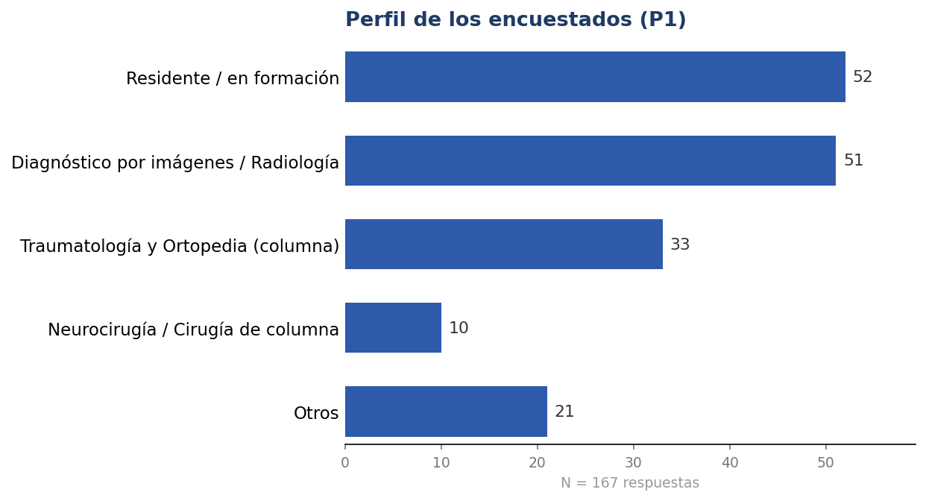
\includegraphics[width=0.92\textwidth]{images/user_research/fig_08_01_encuesta_p1.png}
\vspace{0.4em}

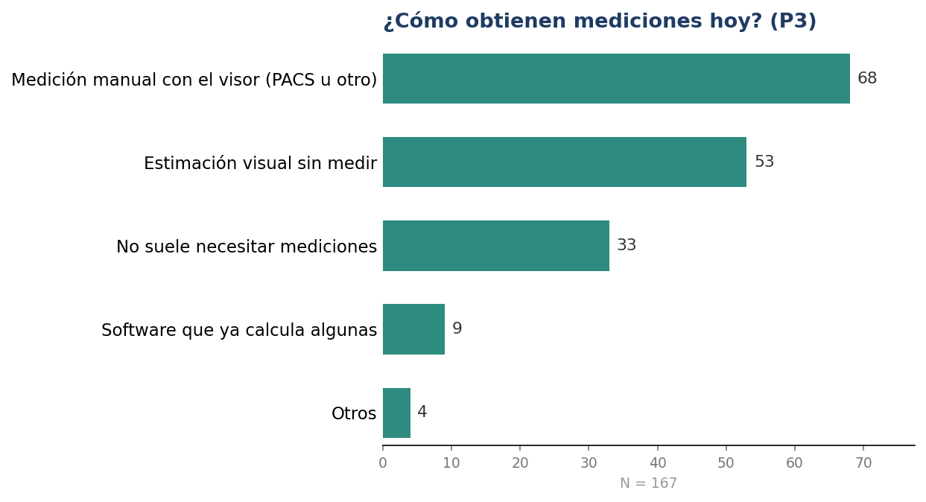
\includegraphics[width=0.92\textwidth]{images/user_research/fig_08_01_encuesta_p3.png}
\caption{Perfil de los encuestados (pregunta 1) y obtención de mediciones en el flujo actual (pregunta 3). Fuente: elaboración propia sobre la encuesta.}
\label{fig:encuesta-p1-p3}
\end{figure}

La utilidad percibida de la segmentación automática es alta y se concentra en las estructuras que el prototipo segmenta: el 81 % considera útil delimitar el canal espinal y el 80 % los discos intervertebrales, mientras que los cuerpos vertebrales obtienen una valoración menor. Sobre qué hace confiable a una segmentación automática, el requisito más votado por amplio margen es poder corregir la segmentación manualmente, seguido de que el sistema exponga un indicador de confianza por estructura. Ese resultado coincide con lo que las entrevistas ya habían señalado y sostiene la decisión de diseño de mantener la revisión profesional como condición de uso y no como funcionalidad opcional.

\begin{figure}[htbp]
\centering
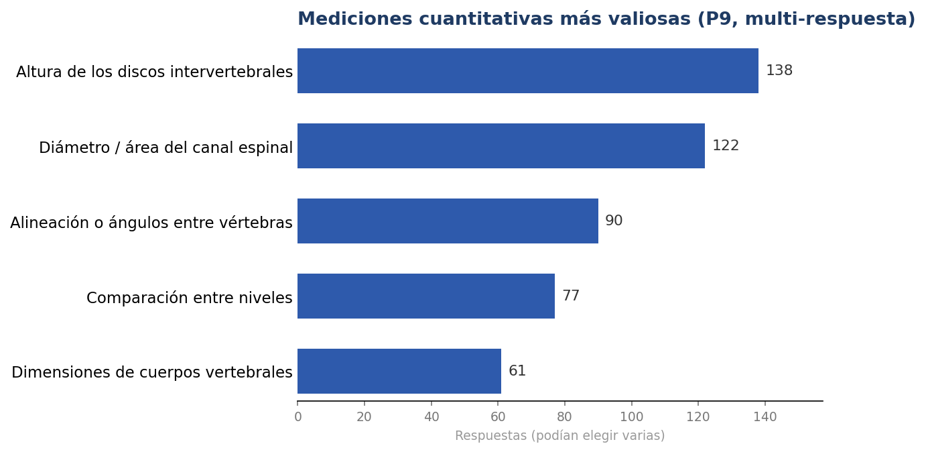
\includegraphics[width=0.92\textwidth]{images/user_research/fig_08_02_encuesta_p9.png}
\vspace{0.4em}

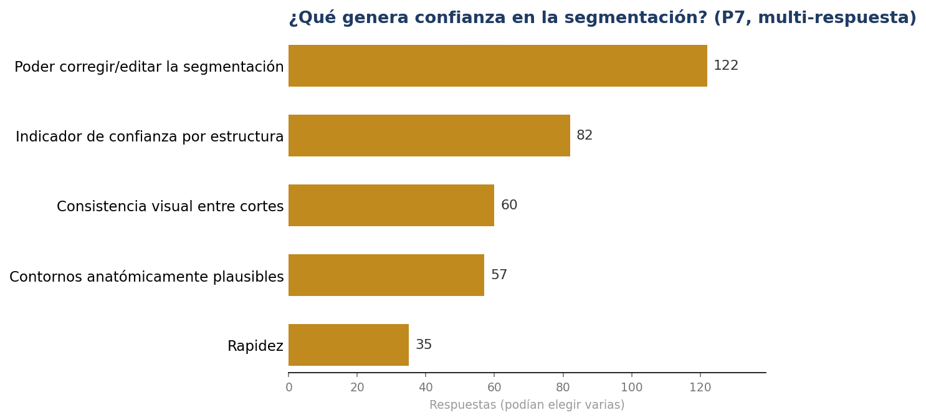
\includegraphics[width=0.92\textwidth]{images/user_research/fig_08_02_encuesta_p7.png}
\caption{Mediciones cuantitativas más valiosas (pregunta 9) y requisitos de confianza en la segmentación (pregunta 7). Fuente: elaboración propia sobre la encuesta.}
\label{fig:encuesta-p9-p7}
\end{figure}

Las afirmaciones sobre transparencia obtuvieron los niveles de acuerdo más altos de la encuesta: el 86 % valora que el sistema explicite cómo llega a un resultado y el 82 % confía más en una herramienta que se presenta como apoyo y no como reemplazo. La disposición a incorporarla al flujo alcanza el 74 %, y las barreras principales son la falta de validación clínica y la dificultad de integración con los sistemas existentes. Ambas barreras corresponden a exclusiones que el Capítulo 5 declara de forma explícita.
% CROSS_REFERENCE_MAPPING_REQUIRED

\begin{figure}[htbp]
\centering
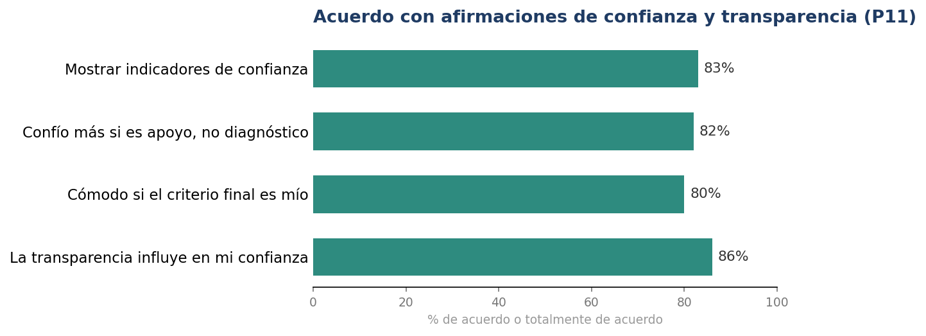
\includegraphics[width=0.92\textwidth]{images/user_research/fig_08_03_encuesta_p11.png}
\vspace{0.4em}

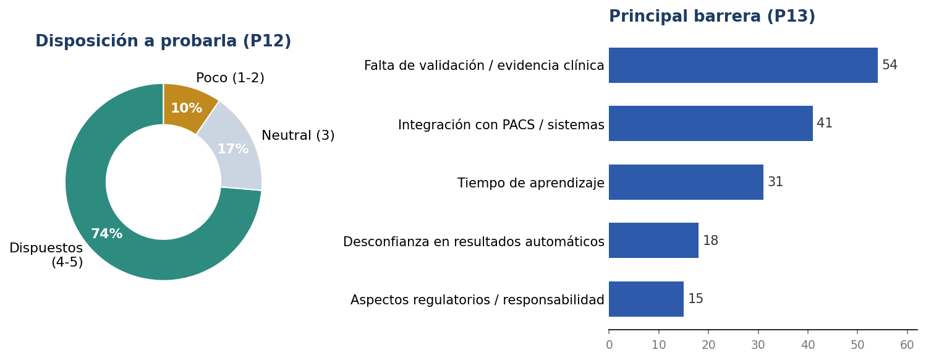
\includegraphics[width=0.92\textwidth]{images/user_research/fig_08_03_encuesta_p12_p13.png}
\caption{Acuerdo sobre confianza y transparencia (pregunta 11), disposición a adoptarla (pregunta 12) y principales barreras (pregunta 13). Fuente: elaboración propia sobre la encuesta.}
\label{fig:encuesta-p11-p12-p13}
\end{figure}
% STRUCTURE_REVIEW_REQUIRED
% DOCX_INLINE_TEXT_AFTER_CAPTION: ### 8.11.3 Síntesis de la encuesta

\subsection{Síntesis de la encuesta}
% STRUCTURE_REVIEW_REQUIRED

La encuesta refuerza cuantitativamente los hallazgos de las entrevistas. Confirma que la cuantificación actual es mayormente manual o visual, que la segmentación y las mediciones aportan valor percibido, y que la adopción depende de la edición humana, los indicadores de confianza, la transparencia y el carácter no diagnóstico de la herramienta. Las barreras señaladas (validación clínica e integración) coinciden con las exclusiones y los trabajos futuros ya documentados. Las 167 respuestas obtenidas constituyen el corte consolidado que acompaña la entrega del 50 %.

\section{Conclusión del capítulo}

El relevamiento permitió validar la pertinencia del proyecto y ajustar su alcance. La incorporación del plano axial es el cambio más visible: dejó de ser una observación del estado del arte para constituir una necesidad funcional detectada en usuarios. La encuesta confirmó cuantitativamente los hallazgos cualitativos y aportó un dato que condiciona el diseño: el requisito más votado para confiar en una segmentación automática es poder corregirla manualmente.

Los hallazgos se formalizan en el Capítulo 9 como requerimientos con criterio de aceptación y trazabilidad hasta su origen. Ninguna de las dos instancias constituye validación clínica: la evaluación con profesionales sobre el producto integrado permanece pendiente.
% CROSS_REFERENCE_MAPPING_REQUIRED
